% =============================================================================
% Plantilla de POSTER — Laboratorio 4: Capa de Red (OMNeT++)
% Cátedra de Redes y Sistemas Distribuidos — FaMAF/UNC
% =============================================================================

\documentclass[final]{beamer}

\usepackage[size=a0,orientation=portrait,scale=1.14]{beamerposter}
\usepackage[T1]{fontenc}
\usepackage[utf8]{inputenc}
\usepackage{lmodern}
\renewcommand{\familydefault}{\sfdefault}
\usepackage{graphicx}
\usepackage{booktabs}
\usepackage{amsmath}
\usepackage{tikz}
\usepackage{pgfplots}
\usepackage{colortbl}
\pgfplotsset{compat=1.18}
\usetikzlibrary{arrows.meta,calc,positioning,shapes.geometric}

% --- Datos del grupo ------------------------------------------------------------
\newcommand{\TituloPoster}{Routing Strategies for Ring Topologies}
\newcommand{\TituloPosterLinea}{in OMNeT++}
\newcommand{\IntegrantesPoster}{Bosque, Lissandro \quad $\bullet$ \quad Galassi, Franco \quad $\bullet$ \quad Pairetti, Joaquín}
\newcommand{\GrupoPoster}{Grupo 31}
\newcommand{\LogoUNC}{figuras/logos/unc-escudo-famaf.png}
\newcommand{\LogoFAMAF}{figuras/logos/logo-famaf.png}

% --- Paleta ---------------------------------------------------------------------
\definecolor{FamafPrimary}{HTML}{0B8BAB}
\definecolor{FamafDark}{HTML}{064F63}
\definecolor{FamafLight}{HTML}{E8F5F9}
\definecolor{FamafAccent}{HTML}{E8A838}
\definecolor{TextDark}{HTML}{2C3E50}
\definecolor{RowShade}{HTML}{D6EEF5}

% --- Estilo beamer --------------------------------------------------------------
\usetheme{default}
\setbeamercolor{headline}{bg=FamafDark,fg=white}
\setbeamercolor{author in head/foot}{bg=FamafDark,fg=white}
\setbeamercolor{block title}{bg=FamafPrimary,fg=white}
\setbeamercolor{block body}{bg=FamafLight,fg=TextDark}
\setbeamercolor{item}{fg=FamafPrimary}
\setbeamercolor{block alerted title}{bg=FamafAccent,fg=white}
\setbeamercolor{block alerted body}{bg=FamafLight,fg=TextDark}

\setbeamerfont{title}{size=\VeryHuge,series=\bfseries}
\setbeamerfont{author}{size=\Large}
\setbeamerfont{block title}{size=\LARGE,series=\bfseries}
\setbeamerfont{block alerted title}{size=\LARGE,series=\bfseries}
\setbeamerfont{block body}{size=\large}
\setbeamerfont{itemize/enumerate body}{size=\large}

% --- Encabezado con banda de acento ---------------------------------------------
\setbeamertemplate{headline}{%
  % Banda superior de acento
  \begin{beamercolorbox}[wd=\paperwidth,ht=0.55cm]{block alerted title}
  \end{beamercolorbox}%
  % Cuerpo del encabezado
  \begin{beamercolorbox}[wd=\paperwidth,leftskip=1.6cm,rightskip=1.4cm,sep=0.65cm]{headline}
    \begin{columns}[c,totalwidth=\textwidth]
      \begin{column}{0.13\textwidth}
        \centering
      \includegraphics[height=7cm,keepaspectratio]{\LogoUNC}
      \end{column}
      \begin{column}{0.70\textwidth}
        \centering
        {\fontsize{44}{52}\selectfont\bfseries \TituloPoster\par}
        \vspace{0.2cm}
        {\fontsize{52}{58}\selectfont\bfseries\textcolor{FamafAccent}{\TituloPosterLinea}\par}
        \vspace{0.35cm}
        {\LARGE\textbf{Laboratorio 4 — Capa de Red}\par}
        \vspace{0.45cm}
        {\Large\IntegrantesPoster\par}
        \vspace{0.2cm}
        {\large\textcolor{white!85}{\GrupoPoster \ $\bullet$ \ FaMAF/UNC \ $\bullet$ \ Redes y Sistemas Distribuidos 2026}\par}
      \end{column}
      \begin{column}{0.13\textwidth}
        \centering
    \includegraphics[height=6.5cm,keepaspectratio]{\LogoFAMAF}      \end{column}
    \end{columns}
  \end{beamercolorbox}%
  % Banda inferior de acento
  \begin{beamercolorbox}[wd=\paperwidth,ht=0.3cm]{block title}
  \end{beamercolorbox}%
}

% --- Pie con banda de acento ----------------------------------------------------
\setbeamertemplate{footline}{%
  \begin{beamercolorbox}[wd=\paperwidth,ht=0.3cm]{block title}
  \end{beamercolorbox}%
  \begin{beamercolorbox}[wd=\paperwidth,leftskip=2.5cm,rightskip=2.5cm,sep=0.7cm,dp=1.2ex]{author in head/foot}
    \begin{columns}[c,totalwidth=\textwidth]
      \begin{column}{0.60\textwidth}
        \Large\textbf{Defensa en clase:} análisis del baseline, diseño del algoritmo propuesto, comparación cuantitativa.
      \end{column}
      \begin{column}{0.38\textwidth}
        \raggedleft\Large
        \textcolor{FamafAccent}{\textbf{FaMAF/UNC}} — Redes y Sist.\ Distribuidos \textbf{2026}
      \end{column}
    \end{columns}
  \end{beamercolorbox}%
  \begin{beamercolorbox}[wd=\paperwidth,ht=0.55cm]{block alerted title}
  \end{beamercolorbox}%
}

\setbeamertemplate{navigation symbols}{}

% ================================================================================
\begin{document}
\begin{frame}[t]

\begin{columns}[T,totalwidth=\paperwidth]

% ==============================================================================
% COLUMNA IZQUIERDA
% ==============================================================================
\begin{column}{0.47\paperwidth}
\hspace{1.5cm}

\begin{block}{Motivación y objetivos}
  \begin{itemize}
    \item \textbf{Problema:} enrutamiento en capa de red con múltiples interfaces en anillo.
    \item \textbf{Baseline:} el kickstarter siempre reenvía por \texttt{lnk[0]} (sentido horario), ignorando el camino más corto.
    \item \textbf{Objetivo:} analizar las limitaciones del baseline, diseñar una estrategia superadora y comparar con datos.
    \item \textbf{Herramienta:} OMNeT++ — 8 nodos, tráfico configurable.
  \end{itemize}
\end{block}

\vspace{0.4cm}

\begin{block}
  \centering\large
  \textit{``Nuestro algoritmo reduce la demora media en \textbf{87\%} y duplica
  el throughput sostenido respecto al kickstarter.''}
\end{block}

\vspace{0.4cm}

\begin{block}{Modelo de simulación}
  \begin{minipage}{0.42\linewidth}
    \centering
    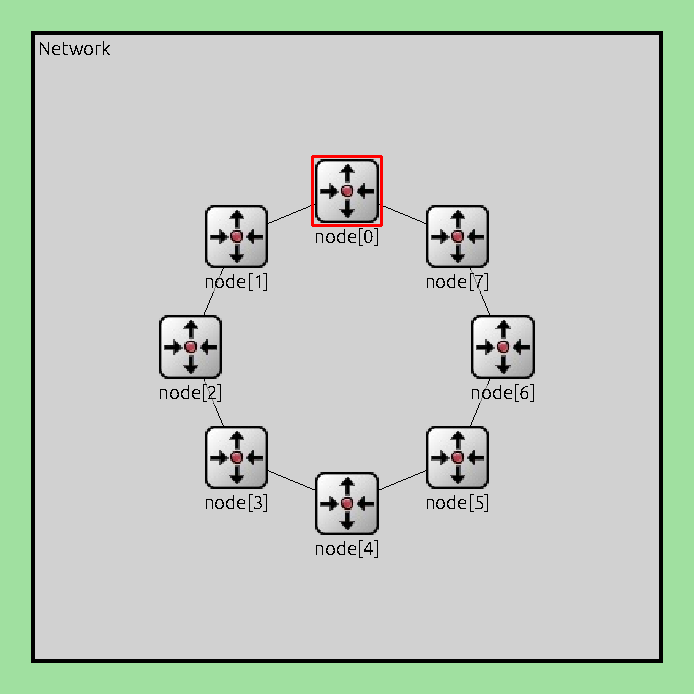
\includegraphics[width=\linewidth]{figuras/topologia-anillo.pdf}
  \end{minipage}
  \hfill
  \begin{minipage}{0.54\linewidth}
    \large
    \textbf{Topología:} anillo de 8 nodos\\
    \quad enlaces full-duplex, 1\,Mbps, delay 100\,µs\\[0.5em]
    \textbf{Capas por nodo:}\\
    \quad \texttt{app} $\to$ \texttt{net} $\to$ \texttt{lnk[0]}, \texttt{lnk[1]}\\[0.5em]
    \textbf{Métricas registradas:}\\
    \quad demora E2E, saltos, buffer, utilización
  \end{minipage}
\end{block}

\vspace{0.4cm}

\begin{block}{Análisis — Caso 1: \texttt{node[0]}, \texttt{node[2]} $\to$ \texttt{node[5]}}
  \centering
  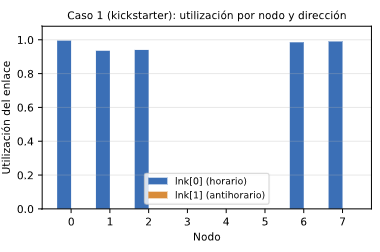
\includegraphics[width=\linewidth]{figuras/caso1.png}

  \vspace{0.5cm}
  \renewcommand{\arraystretch}{1.3}
  \begin{tabular}{@{}lrrr@{}}
    \toprule
    \rowcolor{FamafDark}\textcolor{white}{\textbf{Métrica}} &
    \textcolor{white}{\textbf{Prom.}} &
    \textcolor{white}{\textbf{Máx.}} &
    \textcolor{white}{\textbf{Desv.}} \\
    \midrule
    \rowcolor{RowShade} Demora (s) & 51.16 & 105.56 & 28.31 \\
    Saltos       & 3.92  & 5      & 1.00  \\
    \rowcolor{RowShade} Buffer (pkts) & 91.28 & 190    & 54.83 \\
    Enlace (\%)  & 30.3  & 99.5   & 44.9  \\
    \bottomrule
  \end{tabular}
\end{block}

\vspace{0.4cm}

\end{column}

% ==============================================================================
% COLUMNA DERECHA
% ==============================================================================
\begin{column}{0.5\paperwidth}

\begin{block}{Análisis — Caso 2: 7 fuentes $\to$ \texttt{node[5]}}
  \centering
  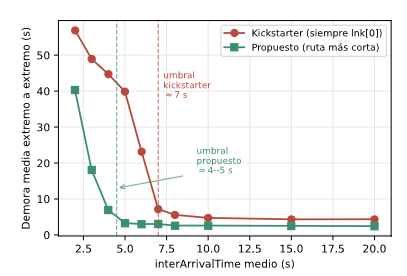
\includegraphics[width=\linewidth]{figuras/caso2.png}

  \vspace{0.3cm}
  \raggedright
  \textbf{Umbral de estabilidad (kickstarter):} \texttt{interArrivalTime} $\approx 7$\,s,
  donde $\rho = \lambda_{\text{total}}/\mu = 7/7 = 1$ en el enlace más cargado.
\end{block}

\vspace{0.4cm}

\begin{block}{Algoritmo propuesto}
  \begin{itemize}
    \item Cada nodo inunda paquetes \texttt{HELLO} (64\,B) por ambas interfaces periódicamente
    \item Al recibir \texttt{HELLO}: aprende ruta si es más corta, reenvía por interfaz opuesta
    \item Al recibir datos: reenvía por la interfaz con menor distancia conocida al destino
  \end{itemize}
  \vspace{0.3cm}
  {\large\ttfamily
  al recibir HELLO (origen s, saltos h, interfaz i):\\[0.1cm]
  \quad si s == miId: descartar\\[0.1cm]
  \quad sino: actualizar tabla si h < mejor conocido\\[0.1cm]
  \quad\quad\quad\, reenviar por (1-i), saltos h+1\\[0.35cm]
  al recibir datos p:\\[0.1cm]
  \quad si dest(p) == local: entregar a app\\[0.1cm]
  \quad sino: reenviar por interfaz de menor distancia
  }
\end{block}

\vspace{0.4cm}

\begin{block}{Evaluación comparativa}
  \begin{minipage}{0.48\linewidth}
    \centering
    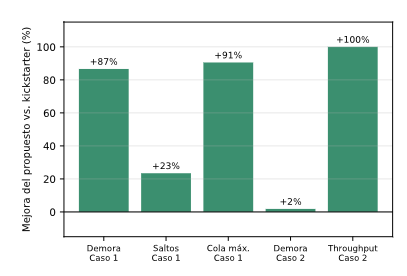
\includegraphics[width=\linewidth]{figuras/comparacion.png}
  \end{minipage}
  \hfill
  \begin{minipage}{0.48\linewidth}
    \centering
    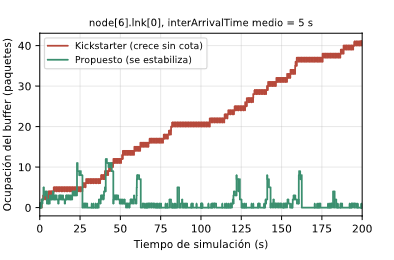
\includegraphics[width=\linewidth]{figuras/tiempo.png}
  \end{minipage}

  \vspace{0.5cm}
  \centering
  \renewcommand{\arraystretch}{1.3}
  \begin{tabular}{@{}lrrrr@{}}
    \toprule
    \rowcolor{FamafDark}
    \textcolor{white}{\textbf{Escenario / Métrica}} &
    \textcolor{white}{\textbf{KS Media}} &
    \textcolor{white}{\textbf{KS Máx.}} &
    \textcolor{white}{\textbf{Prop. Media}} &
    \textcolor{white}{\textbf{Prop. Máx.}} \\
    \midrule
    \rowcolor{RowShade} Caso 1 — Demora (s) & 51.16 & 105.56 & 6.85 & 14.42 \\
    Caso 1 — Saltos       & 3.92  & 5      & 3.00 & 3     \\
    \rowcolor{RowShade} Caso 2 — Demora (s) & 64.53 & 184.23 & 63.35 & 178.56 \\
    Caso 2 — Pkts entregados & 199 & —    & 398  & —     \\
    \bottomrule
  \end{tabular}

  \vspace{0.3cm}
  \raggedright
  \textbf{Bucles:} No — garantizado por construcción (cada HELLO recorre el anillo exactamente una vez).
\end{block}

\end{column}

\end{columns}

\vspace{0.4cm}

% Conclusiones full-width
\begin{beamercolorbox}[wd=\paperwidth,leftskip=1.5cm,rightskip=1.5cm,sep=0.4cm]{block alerted title}
  {\LARGE\bfseries Conclusiones}
\end{beamercolorbox}
\begin{beamercolorbox}[wd=\paperwidth,leftskip=1.5cm,rightskip=1.5cm,sep=0.5cm]{block alerted body}
  \begin{columns}[T,totalwidth=0.93\paperwidth]
    \begin{column}{0.30\linewidth}
      \Large\textbf{Baseline saturado:} el kickstarter concentra los 7 flujos
      en un sentido $\Rightarrow$ $\rho \approx 7$, inestable hasta
      \texttt{interArrivalTime} $\approx 7$\,s.
    \end{column}
    \begin{column}{0.30\linewidth}
      \Large\textbf{Mejora cuantificada:} el algoritmo propuesto reduce la
      demora \textbf{87\%} en Caso~1 y duplica el throughput en Caso~2
      (199 $\to$ 398 paquetes en 200\,s).
    \end{column}
    \begin{column}{0.30\linewidth}
      \Large\textbf{Trabajo futuro:} tolerancia a caídas de nodos
      (expiración de rutas) y generalización a topologías arbitrarias
      con inundación clásica.
    \end{column}
  \end{columns}
\end{beamercolorbox}

\end{frame}
\end{document}
